\begin{center}
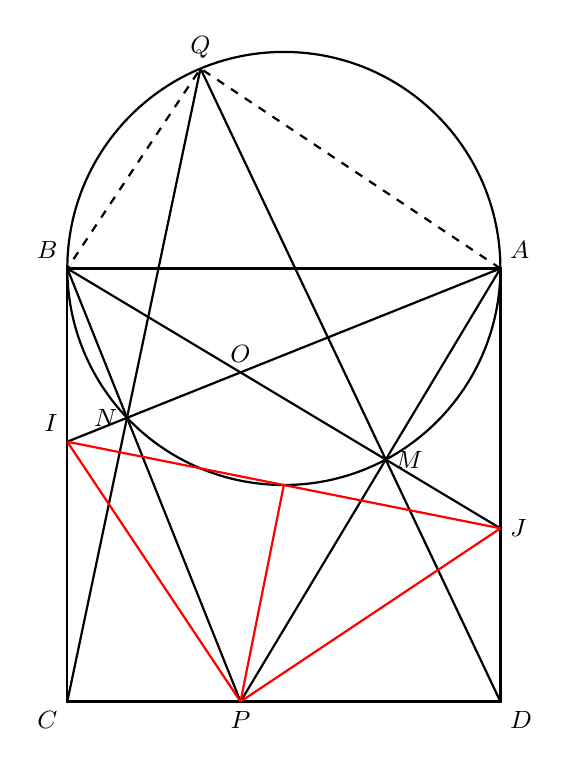
\begin{tikzpicture}[font=\small, scale=1.1]
    % Square ABCD: rotated so AB is top
    \coordinate[label=above right:$A$] (A) at (5,5);
    \coordinate[label=above left:$B$] (B) at (0,5);
    \coordinate[label=below left:$C$] (C) at (0,0);
    \coordinate[label=below right:$D$] (D) at (5,0);

    % Circle K with diameter AB
    \coordinate (CenterK) at (2.5,5);
    \draw[thick] (CenterK) circle (2.5);

    % Point P on CD, P = (2, 0)
    \coordinate[label=below:$P$] (P) at (2,0);

    % M = second intersection of AP with K
    \coordinate[label=right:$M$] (M) at (3.676, 2.794);

    % N = second intersection of BP with K
    \coordinate[label=left:$N$] (N) at (0.690, 3.276);

    % Q = DM \cap CN
    \coordinate[label=above:$Q$] (Q) at (1.538, 7.308);

    % I = AN \cap BC
    \coordinate[label=above left:$I$] (I) at (0,3);

    % J = AD \cap BM
    \coordinate[label=right:$J$] (J) at (5,2);

    % O = center of square ABCD
    \coordinate[] (O) at (2.5,2.5);

    % R = AN \cap BM
    \coordinate[label=above:$O$] (R) at (2,3.8);

    % Draw the square
    \draw[thick] (A)--(B)--(C)--(D)--cycle;

    % Draw lines AP and BP
    \draw[thick] (A)--(P);
    \draw[thick] (B)--(P);

    % Draw lines DM and CN (extended to Q)
    \draw[thick] (D)--(Q);
    \draw[thick] (C)--(Q);
    
    % Draw lines AI (which is AN extended) and BJ (which is BM extended)
    \draw[thick] (A)--(I);
    \draw[thick] (B)--(J);

    % Draw segment IJ in red
    \draw[thick, red] (I)--(J);

    % Draw segments IP, PJ, OP in red
    \draw[thick, red] (I)--(P);
    \draw[thick, red] (P)--(J);
    \draw[thick, red] (O)--(P);

    % Draw AQ and BQ to show angle AQB
    \draw[thick, dashed] (A)--(Q)--(B);

    % Mark right angles at M and N (angle in semicircle)
    % \siku{A}{M}{B}
    % \siku{A}{N}{B}
    % \siku{A}{Q}{B}

    % Draw all points
    % \foreach \s in {A,B,C,D,P,M,N,Q,I,J,O,K,L,R}
    %     \filldraw (\s) circle (1.5pt);
\end{tikzpicture}
\end{center}